
\chapter{Double Integrals}

This chapter covers the following ideas. 

% A list of objectives for the chapter
%\begin{enumerate}
%\item ...
%\end{enumerate}

\begin{enumerate}
\item Explain how to setup and compute a double integrals, as well as
how to interchange the bounds of integration. Use these ideas to find
area and volume.
\item For planar regions, find area, mass, centroids, center of mass,
moments of interia, and radii of gyration.
\item Explain how to change coordinate systems in integration, in
particular to a polar coordinates. Explain what the Jacobian of a
transformation is and how to use it.
\item Explain how to use Green's theorem to compute flow along and
flux across a curve.
\end{enumerate}

%%% Local Variables: 
%%% mode: latex
%%% TeX-master: "../multivariable-calculus"
%%% End: 
%$

\section{Double Integrals}

The integral $\int_a^b fdx$ represents the area of the region in the $xy$
plane above the interval $[a,b]$ along the $x$ axis under the curve
$f(x)$.  We will define a double integral $\iint_RfdA$ in such a
manner to obtain for positive $f(x,y)$ the volume of the solid region
in space above a region $R$ in the $xy$ plane under the surface
$z=f(x,y)$. To start with, we will assume that the region $R$ is a
rectangle $a\leq x\leq b$, $c\leq y\leq d$. Slice the rectangle up into many tiny
rectangles of dimensions $\Delta x_i,\Delta y_j$, making a grid for your region
$R$.  The area of each little subrectangle in the grid is $\Delta A_{ij} =
\Delta x_i\Delta y_j$.  If the grid is made so that $\Delta x_i$ and $\Delta y_j$ are both
really small, then the height of the surface $z=f(x,y)$ above a subrectangle is approximately constant, and can be approximated by the
value of $f$ at some point $f(x_i,y_j)$ in that subrectangle. This
gives an approximation for a small piece of volume as $\Delta V_{ij}\approx
f(x_i,y_j)\Delta A_{ij} = f(x_i,y_j)\Delta x_i\Delta y_j$.  Add up the small pieces
of volume to get total volume as $V\approx \sum_{i=1}^n\sum_{j=1}^m f(x_i,y_j)\Delta
x_i\Delta y_j$.  The double limit $V\approx
\lim_{n\to\infty}\lim_{m\to\infty}\sum_{i=1}^n\sum_{j=1}^m f(x_i,y_j)\Delta x_i\Delta y_j$, if it
exists, is called the double integral of $f$ over $R$, and we write
$\iint_R fdA$. This limit will always exist if the function is
continuous and bounded on $R$.

If a double integral over a rectangle $R$ exists, then it can be
computed using the formulas $\iint_R fdA = \int_a^b \left(\int_c^d f
dy\right)dx = \int_c^d \left(\int_a^b f dx\right)dy$. These last two
integrals are called iterated integrals.  First integrate the inside
integral with respect to the variable inside, then integrate the
result with respect to the outside variable.  

\begin{example}
  For example the integral 
  \begin{align*}
    \int_0^2 \left(\int_1^4 2x+4xy dy\right)dx
  &=\int_0^2 \left( \big[2xy+2xy^2 \big]_{y=1}^{y=4}\right)dx \\
  &=\int_0^2 36x dx =  \big[18x^2\big]_{x=0}^{x=2} \\
  &= 72    
  \end{align*}
gives the same answer as the integral 

\begin{align*}
  \int_1^4\left(\int_0^2 2x+4xy dx\right)dy &= \int_1^4\left(\big[x^2+2x^2y
    \big]_{x=0}^{x=2}\right)dy \\
  &= \int_1^4 4+8ydy = \big[4y+4y^2 \big]_{y=1}^{y=4} \\
  &=
  16+64 - (4 + 4) = 72.  
\end{align*}
\end{example}

The reason a double integral can be computed using either iterated
integral has to do with looking at cross sections.  Rather than
slicing $R$ into a grid using both $\Delta x$ and $\Delta y$, just pick one
direction in which to make slices.  For example, if we cut the region
$R$ along lines parallel to the $y$ axis, then each slice has a width
$\Delta x_i$, and we pick a point $x_i$ in each interval on the $x$ axis.
The area of the cross section of the plane $x=x_i$ under $z=f(x_i,y)$
above the $xy$ plane is given by the integral $A=\int_c^d f(x_i,y)dy$.
Multiply this area $\int_c^d f(x_i,y)dy$ by $\Delta x_i$ for each $i$ to
obtain an approximation for the volume above the $i$th slice of $R$,
i.e. $\Delta V_i\approx \int_c^d f(x_i,y)dy\Delta x_i$. Total volume is found by adding
up the little bits of volume and taking a limit as $\Delta x_i\to 0$. This
gives the volume as 
$V=\int_a^b \left(\int_c^d f dy\right)dx$.  Since the parenthesis take up
extra space, we write simply $\iint_R fdA = \int_a^b \int_c^d f \,dydx = \int_c^d
\int_a^b f \,dxdy$.

If the region $R$ is not a rectangle, but is bounded, and the function
$f$ is bounded for all $(x,y)$ in the region $R$, then we
(theoretically) define the
double integral by placing the region $R$ inside a rectangle which
contains $R$ and defining $f(x,y)=0$ for all $(x,y)$ not in $R$.  To
actually compute the double integral, we pick bounds for the integral which
describe our region.  The outer bounds of the integral must be two
constants. The inner bounds can be functions which involve variables
of the outer bounds.  The outer bounds represent two horizontal or
vertical lines.  The inner bounds represent two functions whose input
is the outer bound variable. 

\begin{example}
\marginpartop{
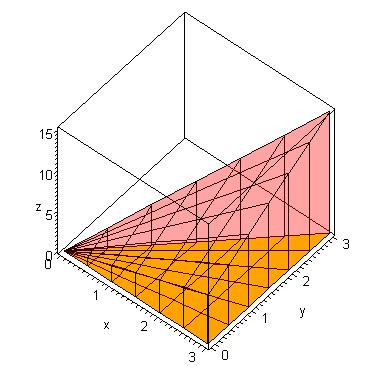
\includegraphics[width=\marginparwidth]{09-DoubleIntegrals/support/double-1}
}%
The volume of the region under the plane $z=2x+3y$ above the region
$R$ which is bounded by the lines $y=x,y=0,x=3$ can be found using a
double integral.  If we choose $y$ as the outer variable, and $x$ as
the inner variable, then we have to pick two constants which trap all
the $y$ values, and then pick two functions of $y$ which trap all the
$x$ values.  The constants are $0\leq y\leq 3$, and the functions are $y\leq x\leq
3$.  The corresponding double integral is $\int_0^3\int_y^3 2x+3y \,dxdy$.
Alternatively, if we choose $x$ as the outer variable and $y$ as the
inner variable, then $x$ is between the constants $0$ and $3$ ($0\leq x\leq
3$) and $y$ is between the functions $y=0$ and $y=x$ ($0\leq y\leq x$).  The
corresponding integral is $\int_0^3\int_0^x 2x+3y \,dydx$. Notice that the
integrand $2x+3y$, the $z$-value being summed, is the same in both
iterated integrals.  The region only affects the bounds of the
integrals and the order of the integration.
\end{example}

If $f=1$, then $\iint_R 1dA$ is the area of the region $R$.  Hence
area (a 2 dimensional quantity) is computed by adding up little bits
of area $dA$.  For the region $a\leq x\leq b$, $0\leq y\leq f(x)$, we have
$\iint_R 1 dA = \int_a^b\int_0^{f(x)}dydx = \int_a^b y\big|_0^{f(x)}dx = \int_a^b
f(x) dx$, which  is the formula found in first semester calculus.


\subsection{Switching the Order of Integration}
Sometimes it is valuable to switch the bounds of integration by
reordering the variables.  This is done by describing the region $R$
(often by constructing a graph), and then changing the way you
describe the region.  

\begin{example}
To compute the integral $\int_0^1\int_y^1
e^{x^2}\,dxdy$, we could first try to integrate the inside integral but
we would fail (as $\int e^{x^2}dx$ does not have an anti-derivative which
is an elementary function). So instead, we write the bounds as
inequalities $0\leq y\leq 1, y\leq x\leq 1$ and realize that the region describe
by these inequalities is the triangle in the first quadrant under the
line $y=x$ for $0\leq x\leq 1$.  Hence we can describe the region also as
$0\leq x\leq 1, 0\leq y\leq x$ which gives the integral $\int_0^1\int_0^x e^{x^2}\,dydx$.
The inner integral is now $\int_0^x e^{x^2}dy = ye^{x^2}\big|_0^x =
xe^{x^2}$.  Hence we have $\int_0^1\int_0^x e^{x^2}\,dydx = \int_0^1 xe^{x^2}dx$,
which is solved by letting $u=x^2$, $du=2xdx$, $dx=\frac{du}{2x}$,
$u(0)=0$, and $u(1)=1$, so $\int_0^1 xe^{x^2}dx = \int_{u=0}^{u=1} x
e^{u}\frac{du}{2x} =  \frac{1}{2}\int_{u=0}^{u=1} e^{u}du =
\frac{1}{2}e^u\big|_0^1 = \frac{1}{2}(e^1-e^0) = \frac{1}{2}(e-1)$.
\end{example}

\begin{example}
The region $R$ inside a circle of radius 3 above the $x$ axis can be
described as either $-3\leq x\leq 3$ and $0\leq y\leq \sqrt{9-x^2}$ or as $0\leq y\leq 3$ and
$-\sqrt{9-y^2}\leq x\leq \sqrt{9-x^2}$.  Hence the integral $\iint_R  1 dA$
can calculated as either $\int_{-3}^{3}\int_{0}^{\sqrt{9-x^2}}dydx$ or
$\int_{0}^{3}\int_{-\sqrt{9-y^2}}^{\sqrt{9-y^2}}\,dxdy$.  Both integrals give
the answer $9\pi/2$, which is the area of this region.  
\end{example}

\begin{example}\label{ex:double-integral}
The integral $\int_0^2\int_{x^2}^{2x}\,dydx$ gives the area of the region
between the curves $y=2x$ and $y=x^2$ and can also be written as
$\int_0^4\int_{y/2}^{\sqrt{y}}\,dxdy$.
\marginpar{
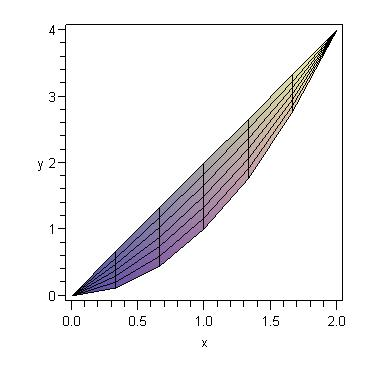
\includegraphics[width=\marginparwidth]{09-DoubleIntegrals/support/double-2}
\centering Example \ref{ex:double-integral}: $\int_0^2\int_{x^2}^{2x}dydx=\int_0^4\int_{y/2}^{\sqrt{y}}\,dxdy$
}%
\end{example}



\section{Changing Coordinate Systems: Generalized $u$-substitution}

To solve the definite integral $\int_0^3 e^{2x}dx$, we make a
substitution $u=2x$ or $x=u/2$, and then notice that $dx =
\frac{1}{2}du$.  Under this substitution, the interval $[0,3]$
transforms to the interval $[0,6]$ and the integral becomes $ \int_0^3
e^{2x}dx = \int_0^6 e^u\frac{1}{2}du$. Notationally, we can write this as
$\int_{C_x} f(x)dx = \int_{C_u} f(x(u))\frac{dx}{du}du$, where $C_x$ and
$C_u$ are the integration bounds in terms of $x$ and $u$ respectively,
and $x(u)=u/2$, so $\frac{dx}{du} = \frac{1}{2}$. Similarly, the
substitution $x=\tan \theta$ gives $\frac{dx}{d\theta}=\sec^2\theta$ and allows us to
compute $\int_0^1\frac{1}{1+x^2}dx =
\int_{0}^{\pi/4}\frac{1}{1+\tan^2\theta}\sec^2\theta d\theta = \int_0^{\pi/4}d\theta = \pi/4$, since
$\tan 0=0$ and $\tan (\pi/4) =1$.

To generalize this to higher dimensions we have to (1) change the
bounds of integration, and (2) replace $\frac{dx}{du}$ with the
generalized version in high dimensions.
To change the bounds in a new coordinate system requires that we
describe the exact same region using different coordinates.  We will
illustrate this with examples.  The term $\frac{dx}{du}$ in higher
dimensions is called the Jacobian of the transformation, and is the
absolute value of the determinant of the derivative of the change of
coordinates. 

\subsection{Polar Coordinates}
Polar coordinates are defined by $x=r\cos\theta, y=r\sin\theta$, which we can
represent using function notation as $T(r,\theta)=\langle r\cos\theta,
r\sin\theta\rangle$. Recall that the derivative of this transformation is 
$DT(r,\theta)= 
\begin{bmatrix}
\cos\theta&-r\sin\theta\\
\sin\theta&r\cos\theta
\end{bmatrix}$. 
The derivative measures small changes in $x,y$ based on small changes
in $r,\theta$.  Determinants calculate area (up to a plus or minus sign).
The determinant of the derivative measures the change in area which
occurs when you change from one coordinate system to another.  To get
a positive value for area, we take the absolute value of the
determinant of the derivative and write $\frac{\partial(x,y)}{\partial(r,\theta)} =
|\det(DT(r,\theta))| = |r\cos^2\theta+r\sin^2\theta| = |r|$. This quantity is called
the Jacobian of the polar transformation from $x,y$ coordinates to $r,\theta$
coordinates.  As long as $r>0$, we can drop the absolute value and we
have that the Jacobian is $\frac{\partial(x,y)}{\partial(r,\theta)}=r$.  So if we wish to
change from $x,y$ to $r,\theta$ coordinates, we use the formula
$\iint_{R_{xy}} f(x,y)\,dxdy = \iint_{R_{r\theta}}
f(T(r,\theta))\frac{\partial(x,y)}{\partial(r,\theta)}drd\theta =  \iint_{R_{r\theta}} f(T(r,\theta))rdrd\theta $.
In differential form, we can abbreviate this as $dA=dxdy = rdrd\theta$. In
other words, after you change all the $x$ and $y$ terms to $r$ and
$\theta$, you have to multiply the entire expression by $r$.

\begin{example}
The region inside a circle of radius $a$ in the plane is easily
described in polar coordinates as $0\leq r\leq a$ and $0\leq \theta\leq 2\pi$. As a
rectangular integral, we can find the area of a circle by writing
$\int_{-a}^a\int_{-\sqrt{a^2-x^2}}^{\sqrt{a^2-x^2}}1\,dydx$, which is a rather
difficult integral to compute. However if we change to polar
coordinates, then we compute $\int_0^a\int_0^{2\pi}rd\theta dr$ or
$$\int_0^{2\pi}\int_0^ardrd\theta  = \int_0^{2\pi}r^2/2\big|_0^ad\theta  = 2\pi a^2/2 = \pi a^2 $$
rather easily. When regions of integration involve circles or curves
that are easily described in polar coordinates, often a change from
rectangular to polar coordinates is extremely useful. 
\end{example}

\begin{example}\label{ex:polar-integral}
The volume of the region in space in the first octant which is below
the paraboloid $z=9-x^2-y^2$, above the $xy$-plane, and satisfying $x\geq
y$, can be found using the iterated double integral $$\iint_R 1 dA =
\int_{0}^{3/\sqrt{2}}\int_{x}^{\sqrt{9-x^2}}9-x^2-y^2\,dydx.$$
 The region $R$
in the $xy$ plane is described in polar coordinates more simply as $0\leq
\theta\leq \pi/4$ and $0\leq r\leq 3$. Changing to polar coordinates we have $z=9-(x^2+y^2)
= 9-r^2$ and then we compute the volume as $V=\int_0^{\pi/4}\int_0^3
(9-r^2)\,rdrd\theta$, which is a much easier integral to compute.
\marginpar{
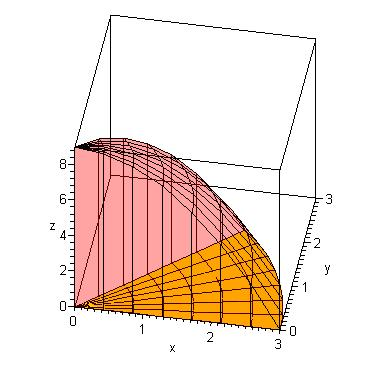
\includegraphics[width=\marginparwidth]{09-DoubleIntegrals/support/polar-1}
\centering Example \ref{ex:polar-integral}
}%
\end{example}

\subsection{General Change of coordinates}

In general, the Jacobian of a transformation $T$ is the absolute value
of the determinant of the derivative of the transformation, often
written $\frac{\partial(x,y)}{\partial(u,v)}$.  Polar coordinates is one of many
standard coordinate systems which people use. Some problems are simple
if you make the right substitution and very difficult if you don't. 
One advantage of working in higher dimensions is that you have the
ability to be creative and find the right change of coordinates to
solve a problem. Here are a few examples.

\begin{example}
To find the area inside of an ellipse
$\frac{x^2}{a^2}+\frac{y^2}{b^2}=1$, use the change of coordinates
$x=au,y=bv$.  The equation of the ellipse becomes $u^2+v^2=1$ in the
$uv$ coordinate system.  The Jacobian of this transformation is
$\left|\det \begin{bmatrix} a&0\\0&b\end{bmatrix}\right|=ab$, so we
have $A = \iint_R dxdy = \iint_{R_{uv}}abdudv = ab\iint_{R_{uv}}dudv$. 
Rather than actually compute the integral, recall that 
$\iint_{R_{uv}}dudv$ is the area of the region in the $uv$ plane,
which is the area inside a circle of radius 1, or $\pi$. Hence the area
of an ellipse is $ab\pi$. If you want a difficult challenge, try
computing this integral without this change of coordinates. 
\end{example}

\begin{example}
\marginpartop{
\aligntop{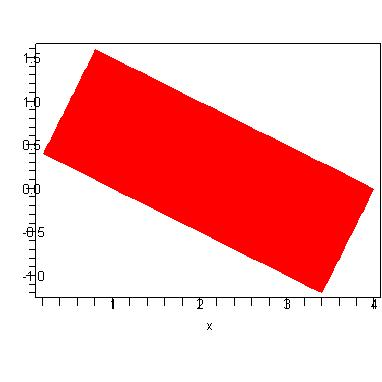
\includegraphics[width=\marginparwidth]{09-DoubleIntegrals/support/general-1}}
}%
If $R$ is the region in the plane bounded by the curves $x+2y=1$,
$x+2y=4$, $2x-y=0$, and $2x-y=8$, and we need to compute the integral
$\iint_R x\,dxdy$, then creating bounds for the integral is a rather
ugly mess.  Instead, we perform the change of coordinates $u=x+2y$ and
$v=2x-y$ (notice that for the first time we have $u$ and $v$ solved in
terms of $x$ and $y$). This change of coordinates transforms us to a
box $[1,4]\times [0,8]$ in the $uv$-plane.  To find the Jacobian of this
transformation, we need to first solve for $x$ and $y$ in terms of $u$
and $v$.  To eliminate $y$, we add $u+2v$ and get $5x$. Similarly,
eliminating $x$ gives $2u-v=5y$, so $x=\frac{u+2v}{5}$ and
$y=\frac{2u-v}{5}$.  The Jacobian of this transformation is
$$\left|\det \begin{bmatrix}
    1/5&2/5\\2/5&-1/5\end{bmatrix}\right|=\left|-1/25-4/25\right|=\left|-1/5\right|=1/5$$
(don't forget the absolute value).  Hence we have $$\iint_{R_{xy}}x\,dxdy
= \int_1^4\int_0^8\frac{u+2v}{5}\left(\frac{1}{5}\right)\,dvdu,$$ which is now
a fairly simple integral to compute.  The right change of coordinates
can simplify a problem.
\end{example}

In the previous problem, to find the Jacobian $\frac{\partial(x,y)}{\partial(u,v)}$,
we first solved for $x$ and $y$ in terms of $u$ and $v$. The ``Inverse
Function Theorem'' implies that $\frac{\partial(x,y)}{\partial(u,v)} =
1/\left(\frac{\partial(u,v)}{\partial(x,y)}\right)$. In other words, we could have
found the derivative of the transformation $T(x,y) = \langle u=x+2y,
v=2x-y\rangle$ as $\begin{bmatrix} 1&2\\2&-1\end{bmatrix}$, and then
after noticing that the absolute value of the determinant is $|-5|$,
we would invert this to obtain $\frac{\partial(x,y)}{\partial(u,v)} = \frac{1}{5}$.  So
you can either solve for $x$ and $y$ first, and then take the
determinant, or you can take the determinant and then invert the
result.  You get the same answer either way.


\section{Physical Applications}
Integrals are used in a wide variety of applications.  You should
notice that in most of the applications below, a formula which works
for double integrals is the same as the integral which we used for
line integrals.  The differentials $dx,ds,dA$ remind us which
dimension we are working in.  For lack of a better notation,  I will
use $d\square$ to represent any of these differentials when you are
free to pick the needed differential. The material which follows is
very similar to the work we did in the line integrals section. I start
by giving a summary of the differential formulas, and then we will use
them to find physical quantities.
\begin{itemize}
\item Area: $dA = fdx,fds, dxdy, rdrd\theta, \frac{\partial(x,y)}{\partial(u,v)}dudv$, 
\item Volume: $dV = fdA$, 
\item Average Value: $(\bar f)\square = \int fd\square$, 
\item Mass: $dm = \delta d\square , \delta dx, \delta ds, \delta dA$
\item Center of Mass: $(\bar x,\bar y,\bar z)m = \int\langle x,y,z\rangle
dm$, where $\int \bar x dm = \int x dm$ is a first moment of mass
\item Moment of Inertia: $I = \int r^2 dm$ is a moment of inertia, and $\int
R^2 dm = \int r^2 dm$ gives $R^2 m =I$ or $R=\sqrt{I/m}$
\end{itemize}
I strongly suggest that as you do each problem, start from a formula
in differential notation, and then modify it so that you have the
right number of integrals.  If you do this, you will learn how to do
calculus in all dimensions with ease. 

\begin{example}
Consider the region {$R = \{(x,y)\mid 0\leq x\leq 3, 0\leq y\leq x\} $} in the plane
with density function {$\delta(x,y) = x^2+y^2+1$}.  
Area is $A=\int_{0}^{3} \int_{0}^{x} dy dx$. Mass is $m=\iint_R dm=\int_{0}^{3}
\int_{0}^{x} (x^2+y^2+1)dy dx$. We can also compute
\begin{align*}
\bar y &= \frac{\int y dm}{\int dm}= \frac{\iint_R y \delta dA}{\iint_R \delta dA} =
\frac{\int_{0}^{3} \int_{0}^{x} y(x^2+y^2+1)dy dx}{\int_{0}^{3} \int_{0}^{x}
x^2+y^2+1dy dx}\\
R_x &= \sqrt{\frac{\int r^2 dm}{\int dm}} =\sqrt{\frac{\int y^2 dm}{\int dm}} =
\sqrt{\frac{\int_{0}^{3} \int_{0}^{x} y^2(x^2+y^2+1)dy dx}{\int_{0}^{3}
\int_{0}^{x} x^2+y^2+1dy dx}}
\end{align*}
\end{example}

\begin{example}
The temperature of a metal object covering the region {$R = \{(x,y)\mid 0\leq
x\leq 3, 0\leq y\leq x\} $} in the plane is given by {$f(x,y) = x^2+y^2+1$}. 
The area of the region $R$ is $A=\iint_R dA = \int_{0}^{3} \int_{0}^{x} dy
dx$ and the average temperature is $AV=\frac{1}{A}
\displaystyle\int_{0}^{3} \int_{0}^{x} x^2+y^2+1 dy dx$. 
\end{example}

\begin{example}
Consider a metal plate occupying the region in the plane bounded by
the curves {$x=y^2$} and {$y=x$}, with density function {$\delta(x,y) =
xy$}.  The mass of the plate is $m=\iint_R \delta dA = \int_0^1\int_{y^2}^{y}
(xy)\,dxdy$.
\end{example}
\begin{example}
The mass of the region in the plane bounded by the curves {$ x=2y $}
and {$ x=y^2 $}, with density {$ x^2+y^2 $}, is
$m=\int_0^2\int_{y^2}^{2y}(x^2+y^2) \,dxdy$. The center of mass is $\bar x =
\frac{1}{m}\int_0^2\int_{y^2}^{2y} x (x^2+y^2) \,dxdy$ and $\bar y =
\frac{1}{m}\int_0^2\int_{y^2}^{2y} y (x^2+y^2) \,dxdy$.
\end{example}

The centroids of many regions are geometrically obvious (such as the
center of a circle, square, or rectangle).   If a centroid is known,
then you can use this knowledge to simplify many integrals.  For
example, we can compute $\displaystyle \int_0^4\int_0^6 3x+5y \,dydx =
3\int_0^4\int_0^6 x \,dydx + 5\int_0^4\int_0^6 y \,dydx= 3\bar x A +5\bar y A = 3\cdot 2\cdot
24 + 5\cdot 3\cdot 24$, since the centroid of the rectangle $R=[0,4]\times[0,6]$ is
$(2,3)$ with area $24$.   





\section{Green's Theorem}





\subsection{Circulation Density }
Let $C$ be a simple closed curve parametrized so that it is traced
counter-clockwise (i.e., we say it is ``oriented counterclockwise'').
Recall that circulation of $\vec F$ along $C$ is
$\oint_C \vec F \cdot d\vec r$.  We now define circulation density for a vector
field $\vec F(x,y)=\langle M,N\rangle$ in the plane. At the point
$(x,y)$ in the plane, create a circle $C_a$ of radius $a$ centered at
$(x,y)$, where the area inside of $C_a$ is given by $A_a$. The
quotient $\frac{1}{A_a}\oint_{C_a} \vec F \cdot d\vec r$ is circulation per
area.  The limit $\lim_{a\to 0} \frac{1}{A_a}\oint_{C_a} \vec F \cdot d\vec r$ is
called the circulation density of $\vec F$ at $(x,y)$.  It can be
shown that $\lim_{a\to 0} \frac{1}{A_a}\oint_{C_a} \vec F \cdot d\vec r =
N_x-M_y$, and that $C_a$ can be replaced with a square of side lengths
$a$ centered at $(x,y)$ with interior area $A_a$ or any collection of
curves $C_a$ which ``shrink nicely'' to $(x,y)$. Regardless, $N_x-M_y$ is
circulation per unit area.

\begin{example}
For the vector field $\vec F = \langle-y,x\rangle$, the
circulation along a circle of radius $a$ is $2\pi a^2$.  Division by the
area $\pi a^2$ and taking a  limit gives $\lim_{a\to 0}\frac{1}{\pi a^2}2\pi
a^2 = 2$ which equals $N_x-M_y = 1-(-1)=2$.
\end{example}

\subsection{Green's Theorem---Circulation Version }
The idea of circulation density is used to show that circulation along
$C$ can be computed by adding up circulation density times $dA$ in the region
$R$, the interior of $C$.  This result is called Green's Theorem:
 $$\oint_C
\vec F\cdot d\vec r = \iint_R N_x-M_ydA.$$

\begin{example}
The circulation of the vector field $\vec F = \langle y^2,x\rangle$
along the circle of radius $2$ is, by Green's Theorem, $$\iint_R 1-2ydA =
A-2\bar y A = \pi(2)^2-2(0)\pi(2)^2 = 4\pi$$ where $A$ is the area inside the
circle. 
\end{example}
\begin{example}
The circulation of the vector field $\vec F=\langle
-y,0\rangle$ along edge of the triangle with vertices
$(0,0),(4,0),(0,3)$ is, by Green's Theorem, $$\int_C \vec F\cdot d\vec r =
\iint_R 1 dA = \frac{1}{2}(3)(4) = 6,$$ or just the area inside of the
curve.  In fact, the area inside of $R$ is $\int_C \vec F\cdot d\vec r =\int_C -y
dx =\iint_RdA$ for any curve $C$, which means that area can be
computed using a line integral.  A planimeter is a drafting tool which
uses Green's theorem to calculate area of any planar region.

\end{example}

\subsection{Flux Density---Divergence $\nabla\cdot \vec F$}

For a vector field $\vec F(x,y)=\langle M,N\rangle$, we define the flux
density, or divergence, of $\vec F$, as follows.  Recall that flux of
$\vec F$ across $C$ is $\oint_C \vec F \cdot \vec n ds = \oint_C Mdy-Ndx$, where
$\vec n$ is the unit outward pointing normal vector and $C$ is
oriented counter clockwise. At the point $(x,y)$ in the plane, create
a circle $C_a$ of radius $a$ centered at $(x,y)$, where the area
inside of $C_a$ is given by $A_a$. The quotient $\frac{1}{A_a}\oint_{C_a}
\vec F \cdot \vec n ds$ has units flux per unit area.  The limit $\lim_{a\to
  0} \frac{1}{A_a}\oint_{C_a} \vec F \cdot \vec n ds$ is called the flux
density of $\vec F$ at $(x,y)$, or \emph{divergence} of $\vec F$.  It
can be shown that $\lim_{a\to 0} \frac{1}{A_a}\oint_{C_a} \vec F \cdot \vec n ds
= M_x+N_y$, and we write $\text{div} \vec F = M_x+N_y = \nabla \cdot \vec
F$. Just as with circulation density, it can also be shown that $C_a$
can be replaced with a square of side length $a$ centered at $(x,y)$
with interior area $A_a$, or any collection of curves $C_a$ which
"shrink nicely" to $(x,y)$, and you still obtain the divergence (flux
per unit area) as $M_x+N_y$.  The notation $\text{div} \vec F = \nabla \cdot
\vec F = \langle\frac{\partial}{\partial x},\frac{\partial}{\partial y}\rangle\cdot\langle M,N\rangle =
\frac{\partial}{\partial x}M+\frac{\partial}{\partial y}N$ gives a convenient way to remember
divergence.

\begin{example}
As an example, we compute the flux density at $(0,0)$ for the vector
field $\vec F = \langle x,y\rangle$. A circle of radius $a$ has unit
normal vector $\vec n = \frac{\langle x,y\rangle}{|\langle x,y\rangle|}$,
so the flux is $\int_C \langle x,y\rangle\cdot
\frac{\langle x,y\rangle}{|\langle x,y\rangle|}ds 
= \int_C\frac{|\langle x,y\rangle|^2}{|\langle x,y\rangle|}ds=\int_C \sqrt{x^2+y^2}ds 
= a \int_C ds   = a2\pi a$, since the circumference of a circle is $2\pi a$.
The area inside a circle of radius $a$ is $\pi a^2$. Hence $\lim_{a\to
0}\frac{1}{\pi a^2}2\pi a^2 = 2$, which equals $\text{div}\vec F = M_x+N_y
= 1+1=2$. 
\end{example}



\subsection{Green's Theorem---Flux version}

Flux in the plane can also be computed by adding up little bits of
flux, which are found by multiplying flux density by area.  This
gives the flux version of Green's Theorem:
$$ \int_C Mdy-Ndx = \int_C\vec F\cdot \vec n ds = \iint_R \text{div}\vec F dA =
\iint_R \left(M_x+N_y\right) dA $$
for $C$ a simple closed curve with interior $R$ and outward normal
$\vec n$, where $C$ is oriented counter clockwise.

\begin{example}
For the vector field $\vec F = \langle x,y\rangle$, we have $\text{div}\vec F = 2$.
The flux of $\vec F$ across the curve which forms the boundary of the
quarter circle of radius 3 in the first quadrant (it has 3 curves
which form the boundary $C$) is simply $\int_C Mdy-Ndx = \int_C \vec F\cdot \vec
n ds = \iint_R 2 dA = 2A = 2\frac{9\pi}{4} =
\frac{9\pi}{2}$. Alternatively, doing the line integral requires setting
up three integrals. The integrals along the axes are zero because
$\vec F\cdot \vec n = 0$. The non-zero integral is found using the
paramaterization $\vec r(t) = \langle3\cos t,3\sin t\rangle$, and is
$\int_0^{\pi/2}Mdy-Ndx =\int_0^{\pi/2}(3\cos t)( 3\cos t)-(3 \sin t) (-3\sin
t)dt =\int_0^{\pi/2}9dt =\frac{9\pi}{2}$.
\end{example}





\section{Proofs of Green's Theorems}
\subsection{Proof of the Circulation version of Green's Theorem}
Let $\vec F(x,y) = \langle M,N\rangle$ be a vector field in the plane.  Let $C$ be
a simple closed smooth space curve, oriented counterclockwise, whose
interior is $R$.  The circulation of $\vec F$ along $C$ is given by
$\int_C\vec F\cdot d\vec r$. Begin by breaking the region {$R$} into little
rectangular pieces with boundary {$C_{ij}$}, oriented
counterclockwise, and interior with area $\Delta A_{ij}$. If the
rectangular region touches the curve {$C$}, then the boundary contains
a small portion of {$C$}.  Notice that when we add together the
circulation along adjoining rectangles, we calculate the flow along
the common boundary twice, once with each orientation.  The sum of the
circulation along adjacent rectangles equals the circulation along the
exterior of the union of the rectangles. All of the interior integrals
disappear, which means we can calculate total circulation by adding up
the circulation along each $C_{ij}$.
\begin{align*}
\int_C\vec F\cdot d\vec r  
&= \sum\sum\int_{C_{ij}}\vec F\cdot d\vec r  
= \sum\sum \frac{1}{\Delta A_{ij}}\int_{C_{ij}}\vec F\cdot d\vec r \Delta A_{ij}\\
&= \sum\sum \frac{\text{circulation along }C_{ij}}{\Delta A_{ij}} \Delta A_{ij}
 \approx \sum \sum (N_x-M_y) \Delta A_{ij}
\end{align*}
Taking limits gives us Green's Theorem $$\int_C\vec F\cdot d\vec r = \iint_R
\left(\frac{\partial N}{\partial x}-\frac{\partial M}{\partial y}\right) dA = \iint_R
\left(N_x-M_y\right) dA.$$    


\subsection{Proof of the Flux version of Green's Theorem}
We now discuss why Green's theorem (the flux version) works. Let {$
  \vec F(x,y) = \langle M,N\rangle$} be a vector field in the plane. Let {$ C $} be
a simple closed smooth space curve (oriented counterclockwise) whose
interior is {$ R $}. The flux of {$\vec F$} across {$C$} is given by
{$\int_C\vec F\cdot\vec n ds$}, where {$\vec n$} is the unit outward normal
to {$C$}. To find total flux, we add up little bits of flux. Break the
region {$R$} into little rectangular pieces with boundary {$C_{ij}$},
oriented counterclockwise. If the rectangular region touches the curve
{$C$}, then the boundary contains a small portion of {$C$}.  When we
add together the flux across adjoining rectangles, we calculate the
flux along the common boundary twice, once with each orientation. The
sum of the flux across adjacent rectangles is the same as the flux
across the exterior of the union of the rectangles. This means that
the total flux equals the sum of the flux across all the little
rectangles. We now write
\begin{align*}
  \int_C\vec F\cdot \vec n ds  
  &= \sum\sum\int_{C_{ij}}\vec F\cdot \vec n ds 
  = \sum\sum\frac{1}{\Delta A_{ij}}\int_{C_{ij}}\vec F\cdot \vec n ds \Delta A_{ij}\\
  &= \sum\sum \frac{\text{flux across }C_{ij}}{\Delta A_{ij}}  \Delta A_{ij}
  \approx \sum\sum (M_x+N_y) \Delta A_{ij}
\end{align*}
 Taking limits gives us the flux version of Green's Theorem $$\int_C\vec
F\cdot \vec n ds =\iint_R \left(M_x+N_y\right) dA.$$






%%% Local Variables: 
%%% mode: latex
%%% TeX-master: "../multivariable-calculus"
%%% End: 





